
\section{Phase 5 - Supervised Imitation Learning: From Sky to Psyche}


\noindent \textbf{Timeline: January 3 -- January 12, 2026}

The objective of Phase 5 was to synthesize a predictive model capable of replicating the Agent’s decision policy with high fidelity. This phase documents the transition from descriptive discovery to the engineering of a predictive inference engine via a comparative algorithmic tournament.

1. Experimental Design: The Tri-League Architecture
2. Categorical Features Selection
3. Model Tournament



\subsection{Experimental Design: The Tri-League Architecture}
To evaluate the interaction between data representation and model performance, the project utilized three distinct feature sets designated as ``Leagues.'' This framework isolates the impact of expert-led curation versus automated abstraction across different algorithmic families.

\begin{table}[H]
    \centering
    \small
    \begin{tabularx}{\textwidth}{l l r X}
        \toprule
        \textbf{League} & \textbf{Basis} & \textbf{Dims.} & \textbf{Technical Objective \& Alignment} \\
        \midrule
        \textbf{League A} & Wide Set (PCA) & 19 PCs & \textbf{Control Group:} Retains 90\% variance of the original 41-feature set to validate that L1-Lasso pruning did not destroy latent signals. \\
        \addlinespace
        \textbf{League B} & Curated (Raw) & 20 Feat. & \textbf{Interpretability Mandate:} Utilizes raw scaled variables to enable SHAP-based forensics and non-linear geometric splits for tree-based models. \\
        \addlinespace
        \textbf{League C} & Curated (PCA) & 12 PCs & \textbf{Mathematical Purity:} Eliminates multicollinearity via orthogonal components to provide a frictionless environment for linear and Bayesian estimators. \\
        \bottomrule
    \end{tabularx}
    \caption{Tri-League data representations for the algorithmic tournament ($N \approx 4,760$).}
    \label{tab:league_alignment}
\end{table}


\subsection{Geospatial Feature Coalescence}
To minimize cardinality and prevent signal fragmentation, the 73 manual polygons and 45 HDBSCAN clusters were consolidated into a unified spatial taxonomy. Micro-polygons were semantically concatenated into \textbf{42 Macro-Zones} to ensure sufficient observation density ($N$) per category. Final feature assignment (\texttt{final\_zone\_id}) followed a deterministic three-tier cascade:

\begin{itemize}[noitemsep, topsep=3pt]
    \item \textbf{Tier 1 (Manual Priority):} Human-defined Macro-Zone boundaries override density clusters to enforce strategic intent.
    \item \textbf{Tier 2 (Machine Fallback):} HDBSCAN clusters capture hyper-dense infrastructural nodes (\textit{e.g., airport terminals}) located outside manual zones.
    \item \textbf{Tier 3 (Unassigned):} Residual coordinates are explicitly categorized as noise.
\end{itemize}

///// agregar que esto resuelve el problema del hdbscan, al forzar poligonos como el del itesm o el de haciendas que no incluyan zonas próximas (las aguilas; san fernando) que fueron incluidas en hdbscan porque excluidas por el coalesce ////7

\subsection{Categorical Feature Selection}
To finalize the feature matrix for supervised learning, a statistical audit was conducted to measure the predictive utility of all candidate categorical variables. The project utilized \textbf{Mutual Information (MI)} to identify non-linear dependencies and the \textbf{Chi-Squared ($\chi^{2}$)} statistic to evaluate independence between features and the decision target.

\begin{figure}[H]
    \centering
    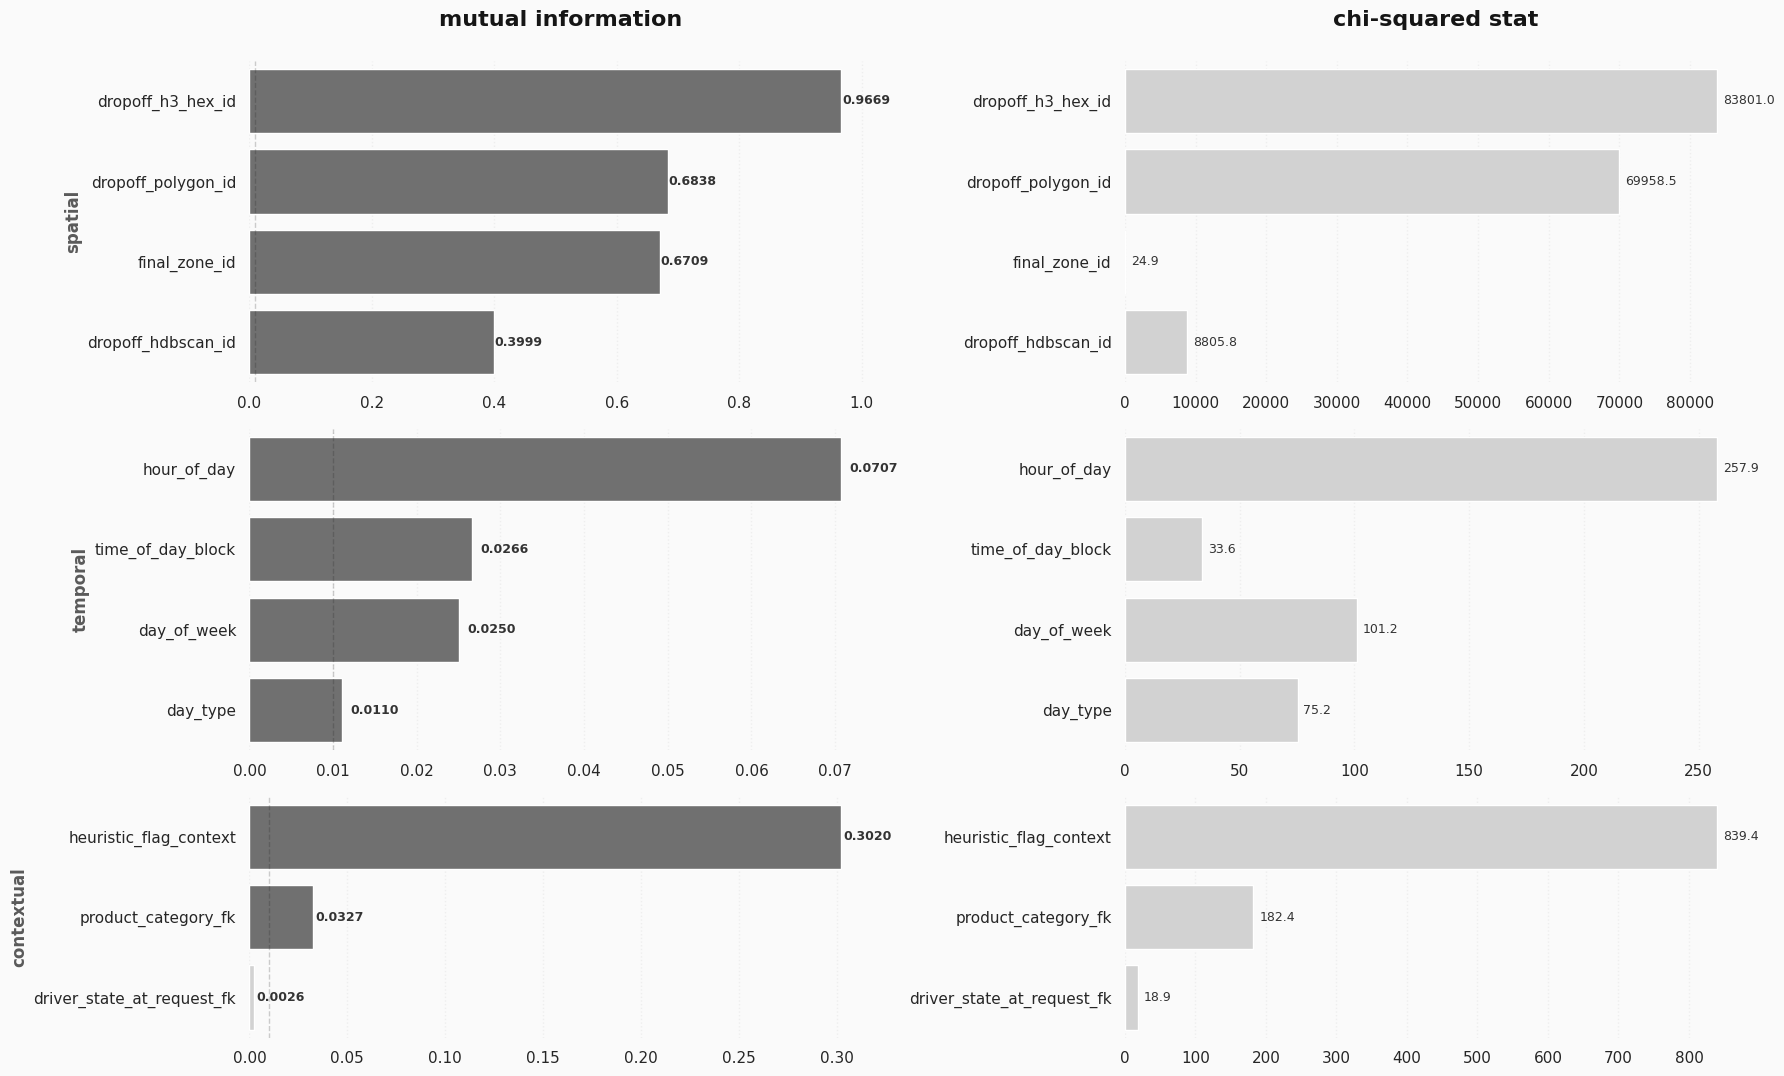
\includegraphics[width=\textwidth]{fig_categorical_audit.png} 
    \caption{Categorical Feature Importance Audit: Mutual Information (Left) and Chi-Squared (Right) scores. The audit exposes the dominance of geospatial topology and the failure of several human-engineered abstractions.}
    \label{fig:categorical_audit}
\end{figure}

The audit identifies \texttt{final\_zone\_id} (MI: 0.671) as the optimal spatial predictor. While high-cardinality grids like H3 with resolution 9 (MI: 0.967) achieve higher raw scores, they risk memorizing the training set. Consolidating 73 polygons into 42 Macro-Zones successfully filtered geometric noise while preserving the variable's predictive power.

The results confirm that raw clock resolution significantly outperforms semantic abstractions. High-resolution features such as \texttt{hour\_of\_day} (MI: 0.071) and \texttt{day\_of\_week} (MI: 0.025) were retained as dominant drivers. Conversely, human-engineered features like \texttt{time\_of\_day\_block} were purged, as their rigid definitions masked critical market variance.

The engineered \texttt{heuristic\_flag\_context} emerged as the primary non-spatial signal (MI: 0.302), validating the "Human-in-the-Loop" extraction phase. In contrast, the Agent's immediate operational state (\textit{Idle vs. On-Trip}) was identified as statistical noise (MI: 0.002) and removed to optimize model focus.

\begin{table}[H]
    \centering
    \small
    \begin{tabularx}{\textwidth}{l l r X}
        \toprule
        \textbf{Domain} & \textbf{Feature} & \textbf{MI Score} & \textbf{Technical Verdict} \\
        \midrule
        \textbf{Spatial} & \texttt{final\_zone\_id} & 0.6709 & \textbf{Keep:} High-resolution zones derived from macro-polygon and cluster coalescence. \\
        \midrule
        \multirow{2}{*}{\textbf{Temporal}} 
        & \texttt{hour\_of\_day} & 0.0707 & \textbf{Keep:} Captures critical high-frequency demand cycles. \\
        & \texttt{day\_of\_week} & 0.0250 & \textbf{Keep:} Preserves unique daily market physics. \\
        \midrule
        \multirow{2}{*}{\textbf{Contextual}} 
        & \texttt{heuristic\_flag\_context} & 0.3020 & \textbf{Keep:} Primary driver; encapsulates strategic intent. \\
        & \texttt{product\_category\_fk} & 0.0327 & \textbf{Keep:} Retained to model service-tier behavioral shifts. \\
        \bottomrule
    \end{tabularx}
    \caption{Final Categorical Feature Set advanced to Supervised Learning ($N \approx 4,760$).}
    \label{tab:cfs_final_set}
\end{table}

\vspace{0.2cm}
\noindent \textit{The high-signal categorical features identified in this audit were integrated into each of the three experimental Data Leagues. This finalized feature space provides the standardized foundation for the subsequent \textbf{Algorithmic Tournament}, where various model architectures are evaluated across these refined data regimes.}


\subsection{Algorithmic Justification: From First Principles to Ensemble Apex}
To identify the optimal architecture for behavioral cloning, a competitive tournament was executed across five developmental trials. Models were evaluated using the \textbf{F1-Macro} score to ensure predictive balance across the 92\% class imbalance.

A priori selection of high-complexity models was rejected in favor of an iterative tournament designed to establish the statistical performance floor and quantify the non-linear complexity of the Agent’s decision policy. This sequence serves as the formal justification for the eventual deployment of gradient-boosted ensembles.

\begin{itemize}[leftmargin=0.5cm, labelsep=0.3cm]
    \item \textbf{Trial 1: Establishing the Statistical Floor (Naive Bayes).} Gaussian Naïve Bayes was deployed to measure performance under the assumption of feature independence. This trial established the baseline "failure rate" for probabilistic models in a high-imbalance, stateful environment.
    
    \item \textbf{Trial 2: Quantifying the Linear Ceiling (Logistic Regression).} By testing linear decision boundaries across both chronological and stratified splits, the project measured the "Linear Limit" of the dataset. 
    
    \item \textbf{Trial 3: The State-Time Tension (LR Stratified).} This controlled test compared chronological purity against stratified data efficiency. It exposed the "shuffling illusion" common in boutique datasets, where over-optimistic scores can mask a failure to generalize to future market regimes.
    
    \item \textbf{Trial 4: Auditing Non-Linear Logic (Decision Tree).} A single tree was utilized as a "Scout" to audit hard logic splits. This trial provided the empirical proof that raw, uncompressed variables (\textit{LIGA B}) significantly outperformed PCA-abstracted features (\textit{LIGA C}) when navigating non-linear decision rules.
    
    \item \textbf{Trial 5: Architectural Apex (XGBoost).} Armed with the quantified proof of non-linearity and the superiority of raw features, the project deployed a gradient-boosted forest on a consolidated five-week "training gym." This finalized the champion architecture required to capture the nuanced interaction between market physics and agent heuristics.
\end{itemize}

\begin{table}[H]
    \centering
    \scriptsize
    \begin{tabularx}{0.9\textwidth}{l l l c c c}
        \toprule
        \textbf{Trial} & \textbf{Algorithm} & \textbf{Validation Method} & \textbf{LIGA A} & \textbf{LIGA B} & \textbf{LIGA C} \\
        \midrule
        1. Floor & Gaussian NB (Hybrid) & Chronological (Custom) & 0.257 & 0.257 & 0.256 \\
        \addlinespace
        2. Linear & Logistic Regression & Time-Series Split & 0.482 & 0.514 & 0.490 \\
        \addlinespace
        3. Theoretical & Logistic Regression & Stratified K-Fold & 0.687 & 0.716 & 0.691 \\
        \addlinespace
        4. Scout & Decision Tree (d=7) & Time-Series Split & 0.336 & 0.474 & 0.373 \\
        \addlinespace
        \textbf{5. Champion} & \textbf{XGBoost Classifier} & \textbf{Stratified K-Fold} & \textbf{0.760} & \textbf{0.761} & \textit{Retired} \\
        \bottomrule
    \end{tabularx}
    \caption{Performance Ledger: F1-Macro averages across the five developmental trials ($N \approx 4,760$).}
    \label{tab:tournament_ledger}
\end{table}


\subsection{Champion Selection: XGBoost}

\subsection{Hyperparameter Calibration: The Down-Tuning Strategy}
Following the identification of \texttt{XGBoost} as the champion architecture, a calibration phase was executed to optimize the model for generalization. The initial \textbf{RandomizedSearchCV} search identified a performance peak at \texttt{max\_depth = 5}, as illustrated in the tuning radiography (Figure \ref{fig:tuning_radiography}). However, subsequent learning curve audits revealed a high-variance gap, suggesting that the model was beginning to overfit the noise of the five-week training window.

To ensure robustness against the unseen Week 6 holdout set, a deliberate \textbf{Down-Tuning} strategy was implemented. By restricting the tree depth and increasing stochasticity, the algorithm was forced to prioritize broad, high-signal features over local data clusters. This increased regularization pressure traded a marginal percentage of training accuracy for a significant improvement in the model's ability to generalize to novel market regimes.

\begin{figure}[H]
    \centering
    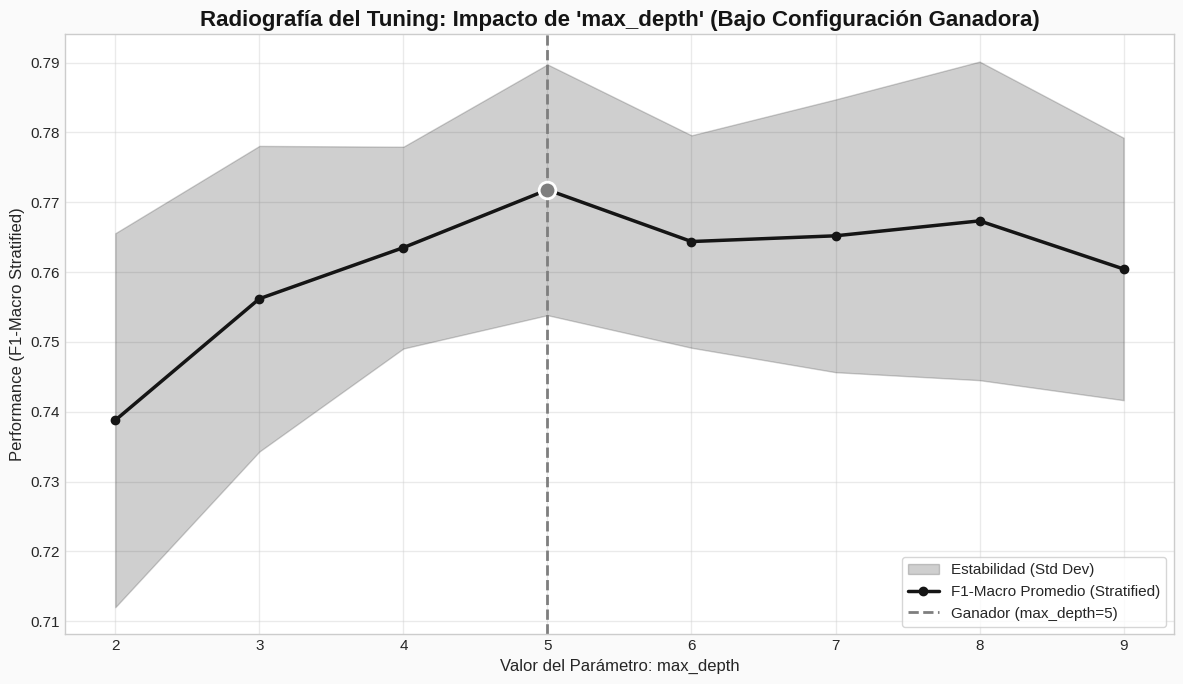
\includegraphics[width=0.9\textwidth]{fig_tuning_radiography.png} 
    \caption{Tuning Radiography: Impact of \texttt{max\_depth} on F1-Macro performance. While the statistical peak occurs at 5, the model was finalized at 4 to ensure defensive generalization.}
    \label{fig:tuning_radiography}
\end{figure}

\begin{table}[H]
    \centering
    \small
    \begin{tabularx}{\textwidth}{l l X}
        \toprule
        \textbf{Hyperparameter} & \textbf{Final Value} & \textbf{Engineering Rationale} \\
        \midrule
        \texttt{n\_estimators} & 200 & Balanced to allow sufficient iterations for convergence at a lower depth limit. \\
        \addlinespace
        \texttt{max\_depth} & 4 & \textbf{Down-Tuned} from 5 to increase regularization and prevent overfitting on small-N zones. \\
        \addlinespace
        \texttt{learning\_rate} & 0.1 & Adjusted to accelerate the learning process within the shallower tree structure. \\
        \addlinespace
        \texttt{subsample} & 0.7 & \textbf{Down-Tuned} from 0.9 to introduce more randomness per tree, forcing reliance on stable global signals. \\
        \addlinespace
        \texttt{min\_child\_weight} & 3 & Enforced to ensure each split is supported by a minimum volume of evidence. \\
        \addlinespace
        \texttt{gamma} & 0.5 & Applied to penalize split complexity and reduce model variance. \\
        \bottomrule
    \end{tabularx}
    \caption{Final \texttt{XGBoost} configuration following the robustness calibration.}
    \label{tab:final_hyperparams}
\end{table}

\subsection{The ``State vs. Time'' Dilemma}
The ``State vs. Time'' dilemma presented a significant architectural trade-off when modeling on a restricted, short-horizon dataset. Enforcing strict chronological purity---such as sequential walk-forward splits across a mere five-week training window---severely restricts the data volume and the number of learning iterations available to the algorithm. The primary limitation encountered was not an uneven distribution of target classes over time, but rather the data starvation inherent to temporal splits on small datasets, which prevents the model from iteratively refining its logic. 

Fortunately, this structural bottleneck was mitigated by the project's pre-existing feature architecture. Because the Agent's temporal context (e.g., \texttt{hour_of_day}, \texttt{day_of_week}) and behavioral memory (e.g., \texttt{consecutive_rejects}, \texttt{accumulated_deadhead}, \texttt{cumulative_earnings}) had already been explicitly engineered into the feature space, the operative "state" and exact temporal positioning of the agent were intrinsically captured within each independent observation; hence, the algorithm does not require sequential chronological ordering to accurately interpret the context of a decision. Consequently, utilizing Stratified K-Fold cross-validation to shuffle the observations within the training pool does not constitute true data leakage. Instead, it serves as a vital architectural mechanism to maximize data efficiency and iterative learning volume, allowing the model to robustly map the stateful logic before facing an untouched, out-of-time evaluation in Week 6.

\subsection{Model Performance: Bimodal Learning}
An audit of the normalized confusion matrix (Figure \ref{fig:monolithic_matrix}) reveals that the monolithic \texttt{XGBoost} champion operates across two distinct performance regimes. These regimes are defined by the degree of feature orthogonality and the presence of deterministic boundaries.

\begin{figure}[H]
    \centering
    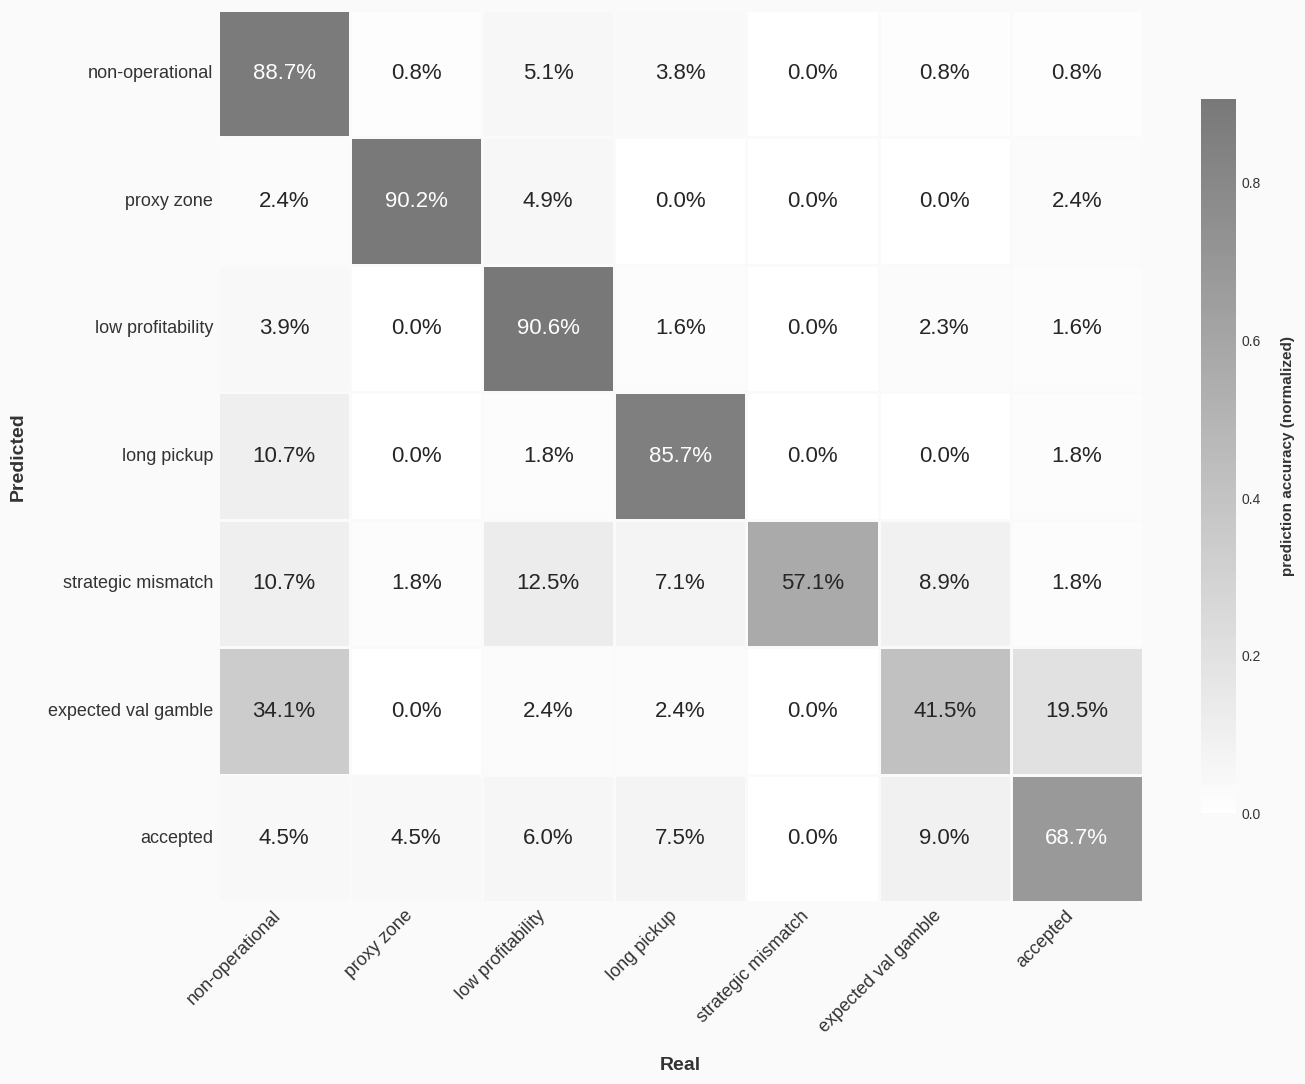
\includegraphics[width=0.85\textwidth]{fig_confusion_matrix_2.png} 
    \caption{Normalized Confusion Matrix for the Monolithic \texttt{XGBoost} Champion. High-accuracy clusters (top-left) identify deterministic operational constraints, while the lower-right quadrant reveals the strategic signal decay in nuanced decision classes.}
    \label{fig:monolithic_matrix}
\end{figure}

\subsubsection{Regime 1: Deterministic Operational Constraints}
The model achieves high accuracy ($>85$\%) when evaluating physical, geographical, and hard-economic constraints: \texttt{proxy\_zone} (90.2\%), \texttt{low\_profitability} (90.6\%), \texttt{non\_operational} (88.7\%), and \texttt{long\_pickup} (85.7\%). These classes are effectively orthogonal; their boundaries are dictated by rigid geospatial coordinates or absolute time-and-fare thresholds. The gradient boosting trees isolate these patterns with minimal entropy, representing the model's "Triage" layer.

\subsubsection{Regime 2: Conditional Strategic Nuance}
Performance degrades significantly ($41\% \dots 68\%$) when the decision boundary shifts to higher-order behavioral states: \texttt{accepted} (68.7\%), \texttt{strategic\_mismatch} (57.1\%), and \texttt{expected\_value\_gamble} (41.5\%). These decisions are not functions of isolated coordinates but involve dynamic calculations of opportunity cost and market velocity. The resulting "fuzzy" boundaries lead to increased entropy and predictive uncertainty.

\subsubsection{The Gravitational Well Effect}
The audit identifies a critical failure mode: the interaction between the majority and minority classes. Because \texttt{non\_operational} constitutes $\approx 50$\% of the dataset, it creates a statistical \textbf{Gravitational Well}. When the algorithm encounters a nuanced observation with high strategic uncertainty---such as an \texttt{expected\_value\_gamble}---it yields to the Bayesian prior of the majority class. This is proven by the fact that \textbf{34.1\% of true strategic gambles are incorrectly swallowed by the non-operational prediction.}


\subsection{Architectural Pivot: The Cognitive Cascade}
The audit confirms that "cheap" triage logic (geospatial/economic filters) cannibalizes "expensive" strategic logic. To eliminate this interference, the project implemented the \textbf{Hierarchical Cognitive Cascade}. This architecture decomposes the multi-class problem into a sequence of specialized inference layers:

\begin{itemize}[noitemsep, topsep=3pt]
    \item \textbf{Layer 1 (The Bouncer):} A classifier designed to remove the "Regime 1" noise (\textit{Non-Op, Proxy, Long Pickup}).
    \item \textbf{Layer 2 (The Strategist):} A secondary model operating strictly on the high-yield, surviving observations.
\end{itemize}

By removing the gravitational pull of the non-operational class in Layer 1, the Strategist model can dedicate its full capacity to resolving the subtle economic differences between strategic rejections and acceptances, effectively breaking the performance ceiling identified in the flat architecture.

\subsection{Layer 1: The Balanced Bouncer Protocol}
Layer 1 is architected as a high-recall filter designed to isolate deterministic operational noise from strategic signal. This "Bouncer" ensures that the majority classes (\textit{Non-Op, Low Profit}) do not overwhelm the more nuanced strategic rejections in the subsequent layer.

\subsubsection{The Threshold Paradox: Street vs. Code}
The calibration of this filter is driven by an identified asymmetry in risk tolerance between the physical agent and the digital system:

\begin{itemize}[noitemsep, topsep=3pt]
    \item \textbf{The Agent (The Street):} Prioritizes the avoidance of \textbf{False Positives} (accepting a "Trap" offer). This results in a high internal threshold and a conservative decision bias.
    \item \textbf{The System (The Code):} Prioritizes the avoidance of \textbf{False Negatives} (discarding a "Super Gem" as noise). Since a lost opportunity is irrecuperable, the system utilizes a low threshold to maximize the volume of nuanced signal passed to Layer 2.
\end{itemize}

\subsubsection{Priority-Based Decision Logic}
To operationalize this strategy, Layer 1 replaces standard $argmax$ classification with a priority-based rule. The predicted class $\hat{y}$ is determined by two calibrated thresholds:

\begin{equation}
\hat{y} = 
\begin{cases} 
\text{Low Profit} & \text{if } P(\text{Low Profit}) \ge 0.25 \\
\text{The Nuanced Rest} & \text{else if } P(\text{Nuanced}) \ge 0.20 \\
\text{argmax}(P) & \text{otherwise}
\end{cases}
\end{equation}

\noindent \textbf{Hierarchy:} Blocking "Low Profit" data always takes precedence over rescuing "Nuanced" signal to enforce economic discipline.

\subsubsection{Results: Filter Efficiency}
The performance of the filter is measured by its \textbf{Recall} (Filter Efficiency). As shown in Figure \ref{fig:layer1_matrix}, the protocol achieved a 90.6\% Recall for Low Profitability rejections and a 81.7\% Recall the Nuanced Rest Class.

\begin{figure}[H]
    \centering
    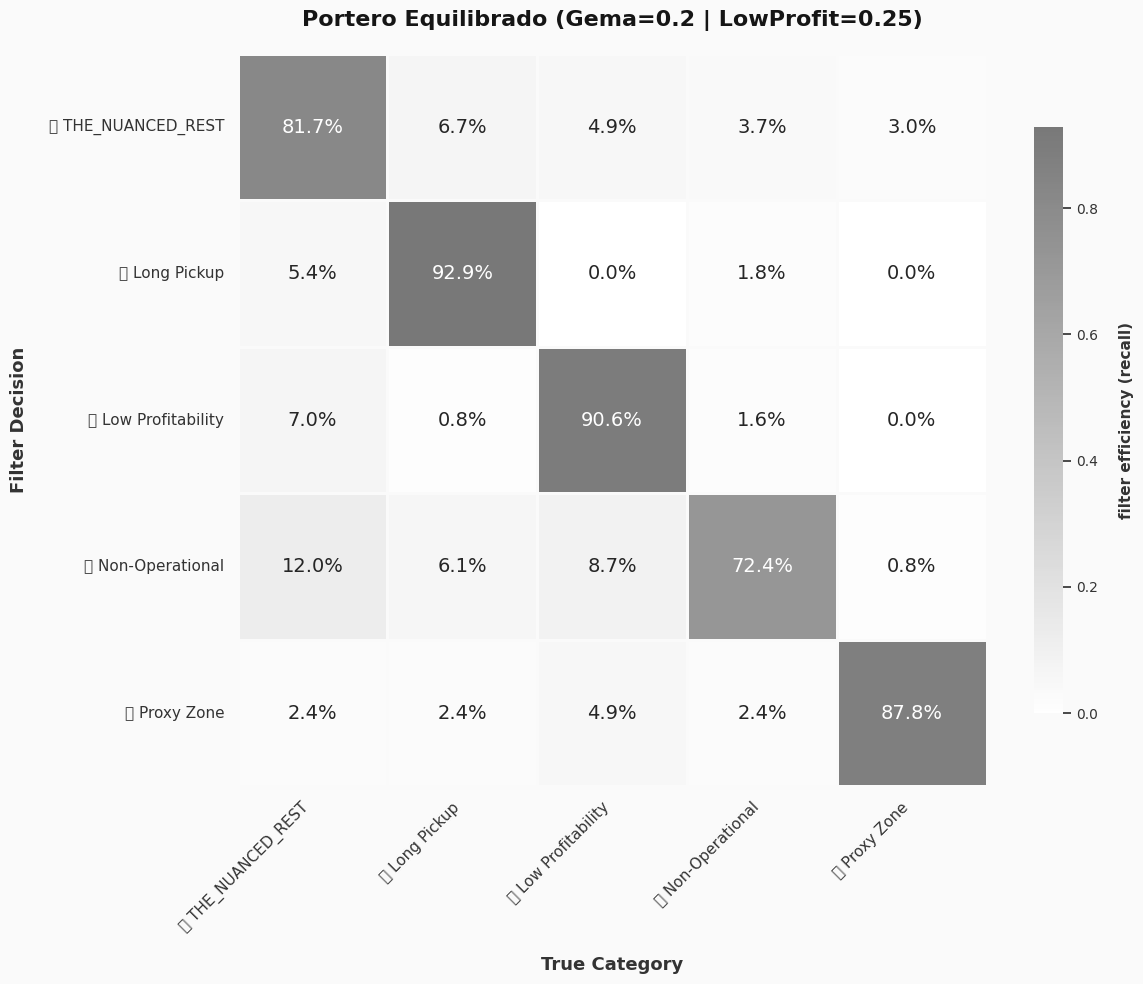
\includegraphics[width=0.8\textwidth]{fig_layer1_matrix.png} 
    \caption{Layer 1 Confusion Matrix. The diagonal represents the filter's efficiency in removing noise, while the "Nuanced Rest" column represents the survival rate of strategic signal.}
    \label{fig:layer1_matrix}
\end{figure}

\noindent \textit{Outcome: By using high-recall filtering, the project successfully neutralized the Gravitational Well. The observations passed to Layer 2 are statistically balanced and represent the true strategic DNA of the expert policy.}

To validate the triage logic of the Balanced Bouncer, a SHAP contribution analysis was executed for the \texttt{THE\_NUANCED\_REST} class. This "DNA Atlas" (Figure \ref{fig:nuanced_dna}) identifies the features that qualify an offer for Layer 2 evaluation (Teal/Right) versus those that push it toward a deterministic rejection (Gray/Left).

\begin{figure}[H]
    \centering
    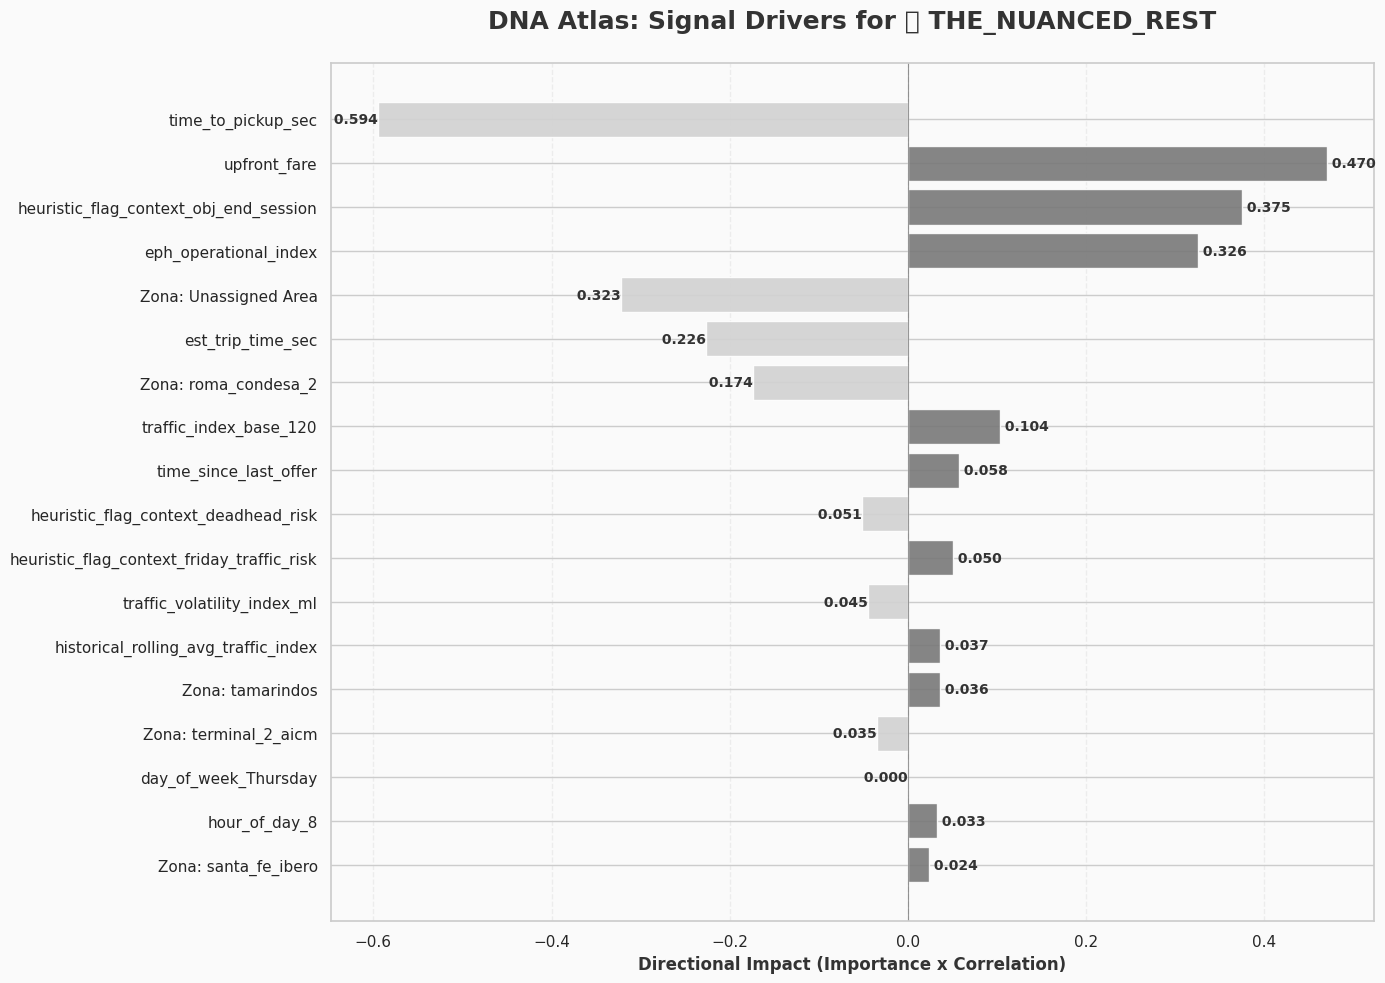
\includegraphics[width=0.75\textwidth]{fig_nuanced_dna.png} 
    \caption{DNA Atlas: Signal Drivers for \texttt{THE\_NUANCED\_REST}. The chart illustrates the contribution of features to the triage decision. Logistical friction serves as the primary exclusion vector, while financial magnitude and strategic intent serve as the primary inclusion vectors.}
    \label{fig:nuanced_dna}
\end{figure}

The analysis reveals three primary pillars governing the triage stage:

\begin{itemize}[noitemsep, topsep=3pt]
    \item \textbf{The Logistical Barrier:} \texttt{time\_to\_pickup\_sec} is the dominant negative driver ($-0.594$). Regardless of potential yield, high pickup latency is the primary reason an offer fails to reach the strategic tier. This confirms the model enforces strict logistical discipline at the entry point.
    
    \item \textbf{The Financial Magnet:} \texttt{upfront\_fare} ($+0.470$) and \texttt{eph\_operational\_index} ($+0.326$) are the primary positive drivers. High absolute and relative earnings are the strongest signals for moving an offer into the nuanced category for strategic evaluation.
    
    \item \textbf{The Strategic Intent Trigger:} The positive contribution of the \texttt{obj\_end\_session} flag ($+0.375$) confirms that the model recognizes the "Endgame" state. When this intent is active, the model categorizes offers as "nuanced" rather than "low profit," allowing the subsequent Layer 2 model to evaluate them against homecoming vectors.
\end{itemize}

\noindent \textit{Outcome: The Layer 1 DNA confirms that the hierarchical filter has successfully learned the Agent's triage logic. By effectively isolating logistical noise and economic failures, the system ensures that Layer 2 operates on a high-signal subset of the marketplace.}



\subsection{Layer 2: The Strategist (Nuance Modeling)}
The second stage of the cascade represents the "Nuance Engine" of the system. Operating exclusively on the high-yield subset that survived the Layer 1 filter, this model is designed to resolve the subtle distinctions between strategic rejections and acceptances without the interference of majority-class noise.

\begin{figure}[H]
    \centering
    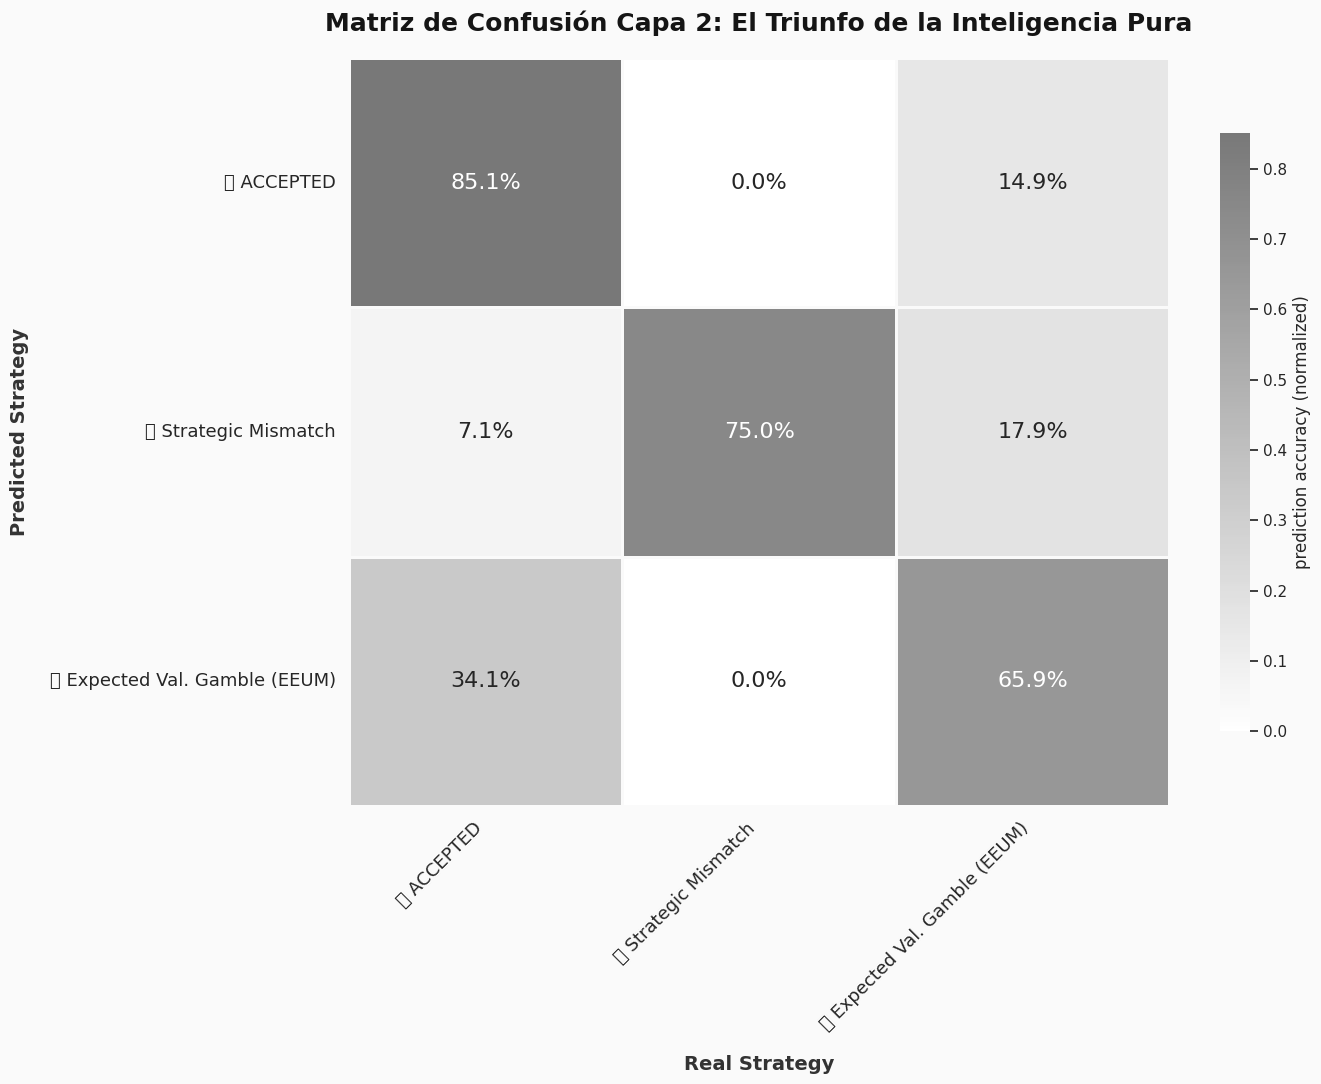
\includegraphics[width=0.75\textwidth]{fig_layer2_matrix.png} 
    \caption{Layer 2 Confusion Matrix. By isolating the high-yield sub-universe, the model achieves superior separation between complex strategic states.}
    \label{fig:layer2_matrix}
\end{figure}

\subsubsection{Results: Strategic Performance Lift}
The transition to a hierarchical architecture resulted in a significant accuracy lift for the strategic classes (Figure \ref{fig:layer2_matrix}):

\begin{itemize}[noitemsep, topsep=3pt]
    \item \textbf{Geospatial Strategy (\texttt{strategic\_mismatch}):} Accuracy reached \textbf{75.0\%}, confirming the model successfully mapped complex heuristics such as "Friday Gridlock Avoidance" and "Non-Homecoming Vectors."
    \item \textbf{Optimal Stopping (\texttt{expected\_value\_gamble}):} Accuracy rose to \textbf{65.9\%}, a 58\% relative improvement over the monolithic baseline. This proves that removing deterministic noise allows the algorithm to better isolate opportunity-cost signals.
    \item \textbf{Primary Target (\texttt{ACCEPTED}):} The model achieved \textbf{85.1\% accuracy} in replicating the Agent’s acceptance decisions, establishing a high-fidelity behavioral clone.
\end{itemize}

\subsubsection{Threshold Tuning and the Pareto Frontier}
A systematic grid search for optimal decision thresholds was conducted for the Strategist layer. However, the analysis identified a sharp **Pareto Frontier**: while the threshold for the \texttt{ACCEPTED} class could be tightened, doing so resulted in a disproportionate collapse of \textit{Recall} for the \texttt{expected\_value\_gamble} and \texttt{strategic\_mismatch} classes. Because the project prioritizes high-fidelity policy replication over raw binary accuracy, the thresholds were maintained at their balanced equilibrium to preserve strategic nuance.



\vspace{0.4cm}
\rule{\linewidth}{0.4pt}


\subsubsection{Strategic DNA: Feature Drivers for Layer 2}
To interpret the internal logic of the Strategist model, a SHAP contribution analysis was performed across the three nuanced strategic classes (Figure \ref{fig:layer2_shap_dna}). This assessment quantifies the directional impact of features on the final classification.

\begin{figure}[H]
    \centering
    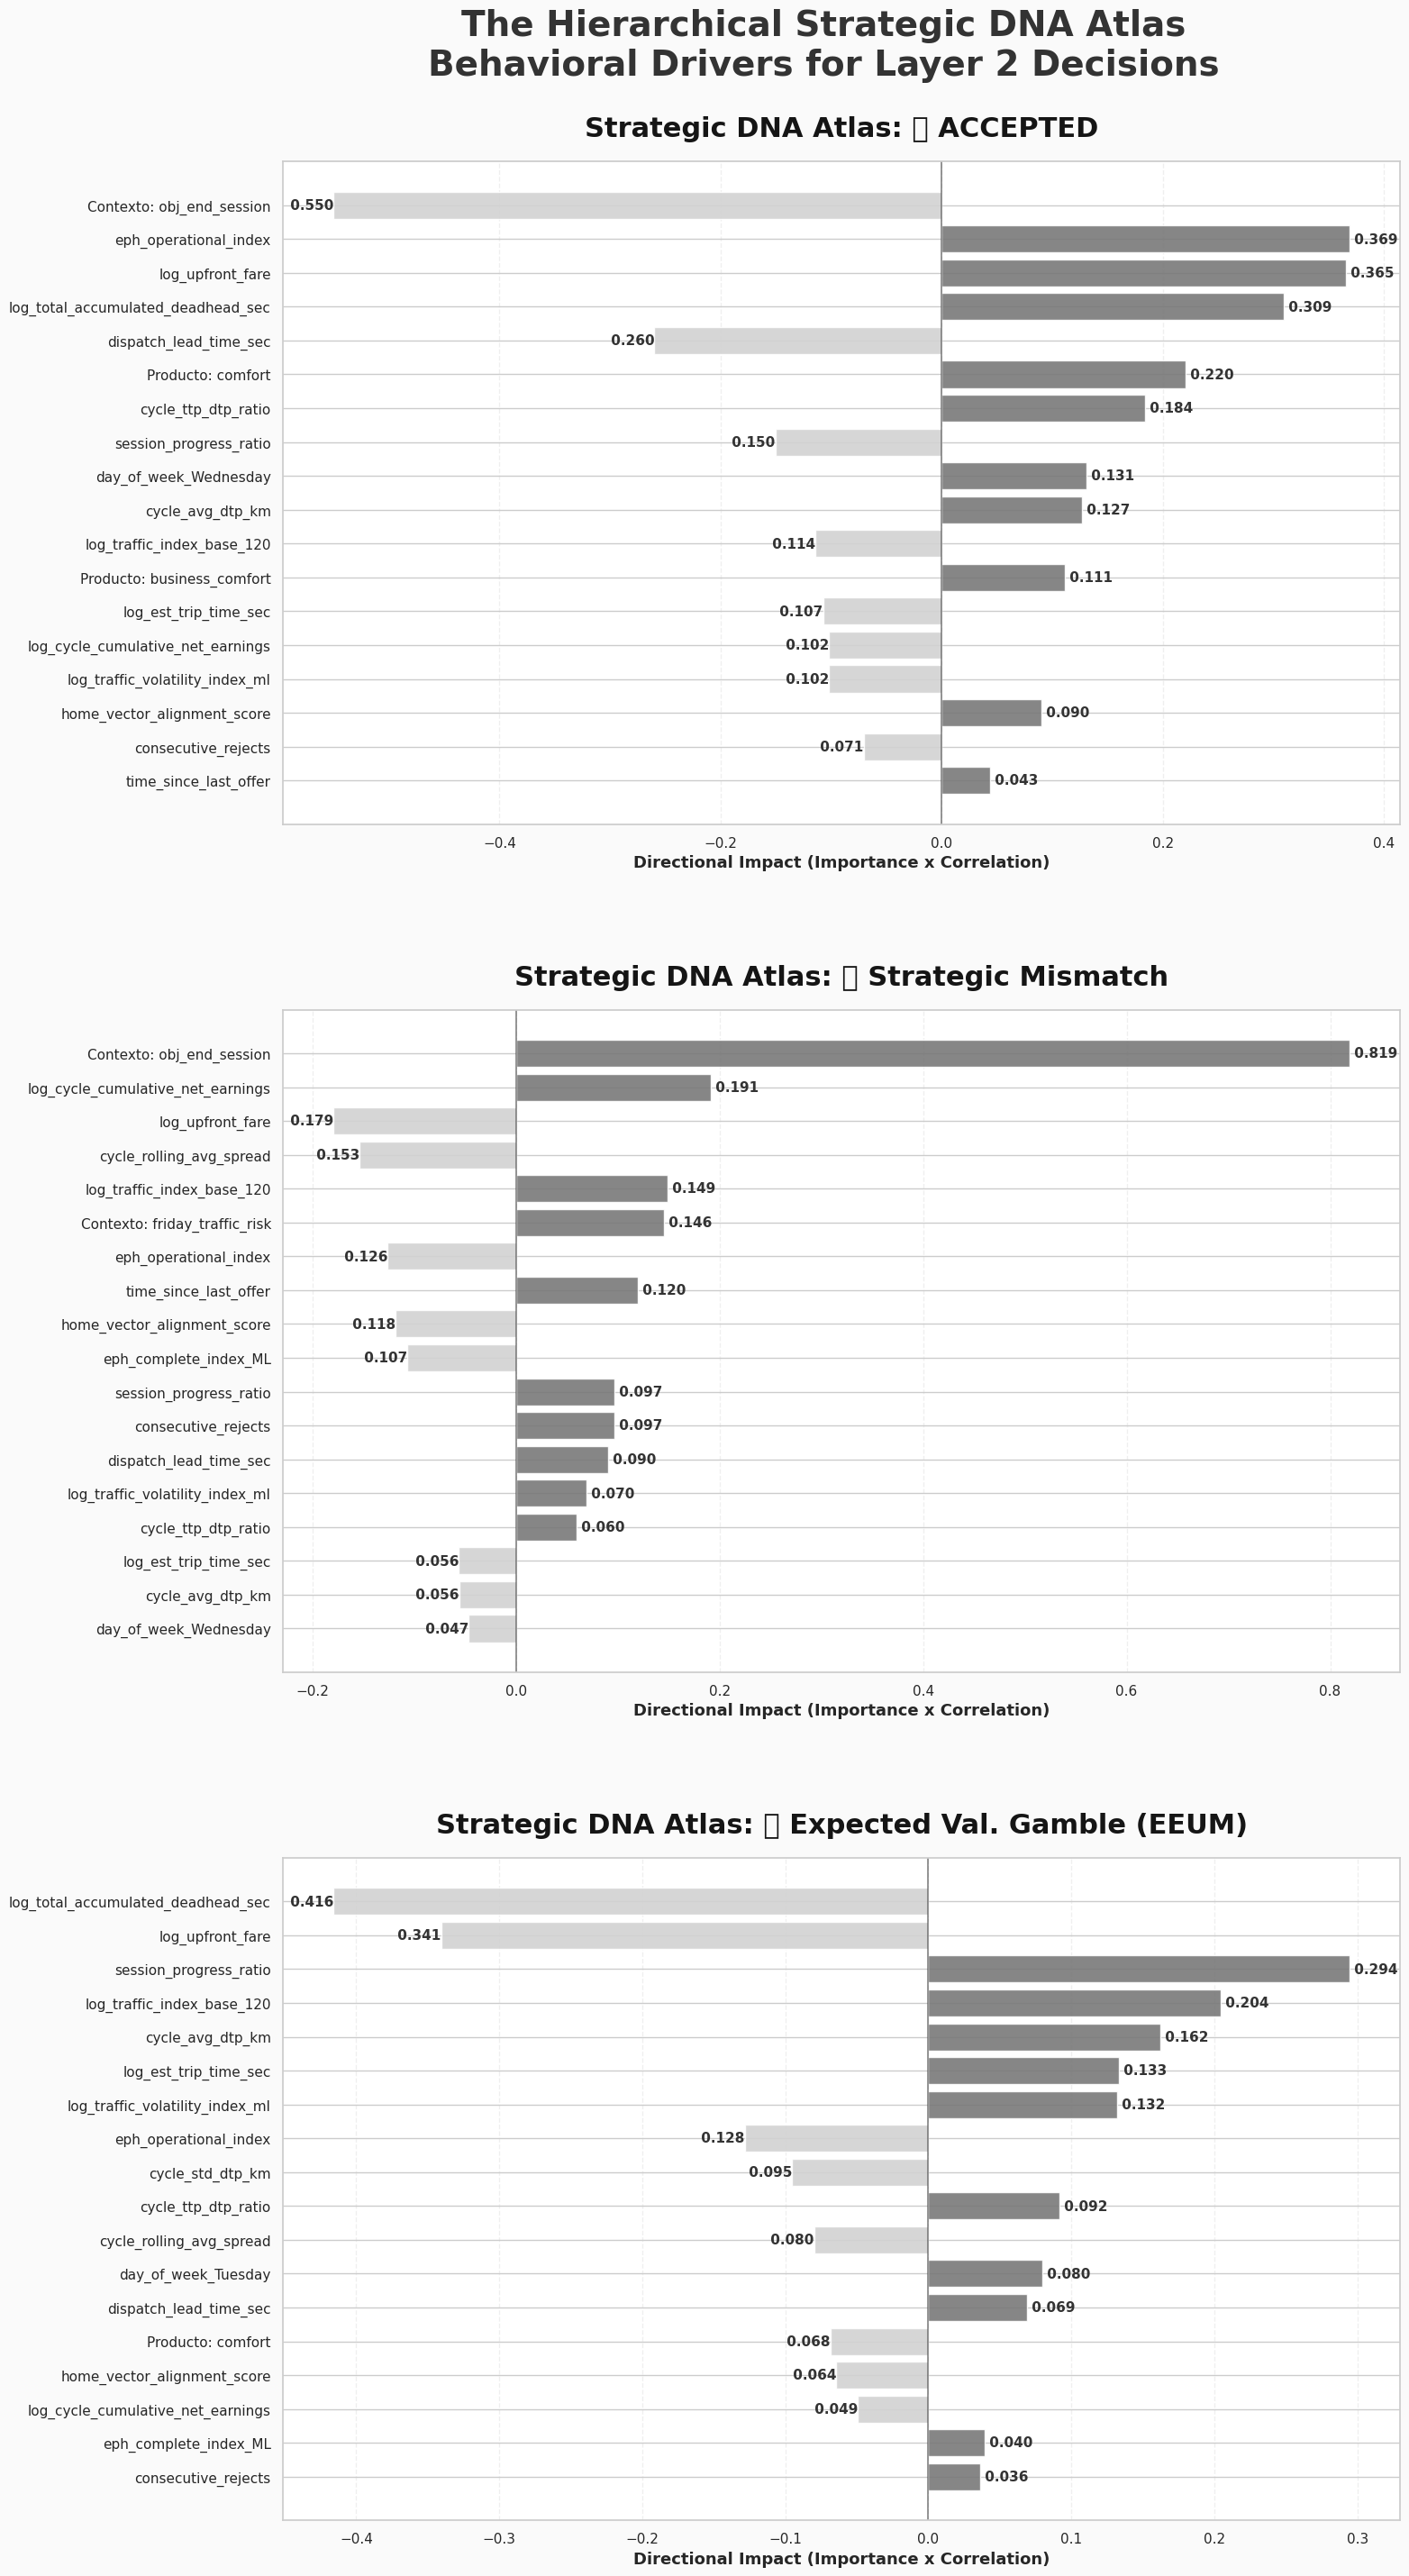
\includegraphics[width=0.6\textwidth]{fig_layer2_shap_dna.png} 
    \caption{Hierarchical Strategic DNA Atlas: Feature contributions for Layer 2 decision classes. Teal bars indicate a positive contribution to class probability; Gray bars indicate a negative contribution.}
    \label{fig:layer2_shap_dna}
\end{figure}

The analysis reveals three primary behavioral mechanics that govern the expert agent's high-level strategy:

\begin{itemize}[noitemsep, topsep=3pt]
    \item \textbf{The Sunk Cost Mechanic (Accepted):} While \texttt{upfront\_fare} and \texttt{eph\_operational\_index} are the expected financial drivers, \texttt{log\_total\_accumulated\_deadhead\_sec} serves as a powerful positive predictor ($+0.309$). This provides empirical proof of a ``Sunk Cost'' effect: as uncompensated search time increases, the Agent's selectivity threshold decays, leading to a higher probability of acceptance. Conversely, \texttt{obj\_end\_session} acts as the strongest inhibitor ($-0.550$), suppressing acceptance regardless of yield.
    
    \item \textbf{The Income Targeting Mechanic (Strategic Mismatch):} This class is dominated by the \texttt{obj\_end\_session} context ($+0.819$). The model correctly identifies that high accumulated earnings (\texttt{log\_cycle\_cumulative\_net\_earnings}) pull the decision toward a mismatch rejection. This verifies the ``Income Targeting'' heuristic: once financial objectives are met, the Agent prioritizes homecoming vectors over marginal revenue gains.
    
    \item \textbf{The Patience Constraint (Expected Val. Gamble):} The primary predictor for the \texttt{expected\_value\_gamble} class is the \textbf{absence} of search fatigue. The strongest negative contributor is \texttt{log\_total\_accumulated\_deadhead\_sec} ($-0.416$). This identifies a critical behavioral constraint: the Agent only gambles on future offers when the current search cost is low. Prolonged search cycles eliminate the Agent's patience, causing a shift from strategic gambling back to acceptance.
\end{itemize}

\noindent \textit{Outcome: The Layer 2 feature assessment proves that the XGBoost champion successfully mapped the Agent's non-linear strategic logic. The quantification of the ``Patience Threshold'' and the ``Sunk Cost Effect'' provides the mathematical foundation for the generative simulation engine in Phase 6.}


\subsection{The Shadow Mode Trial: Behavioral Fidelity}
To measure the operational impact of the architectural pivot, a final performance assessment was executed on the firewalled Week 6 holdout set ($N \approx 780$ offers). The finalized \textbf{Cognitive Cascade} was benchmarked head-to-head against the monolithic \texttt{XGBoost} baseline and the Human Agent’s actual decisions across two primary KPIs: cumulative upfront fare and strategic efficiency.

\begin{figure}[H]
    \centering
    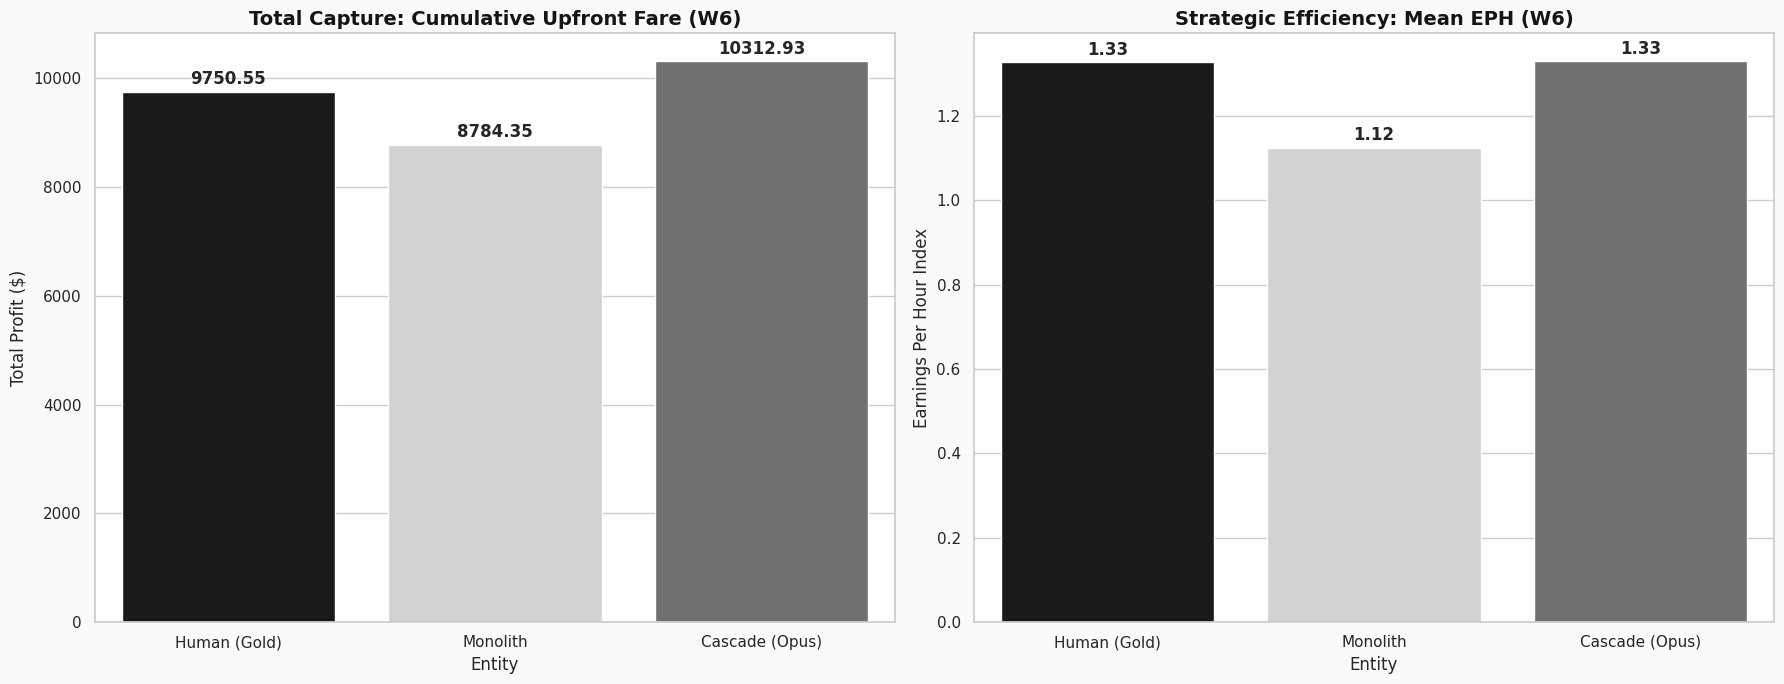
\includegraphics[width=\textwidth]{fig_shadow_mode_results.png} 
    \caption{Shadow Mode Performance Results. The left plot measures total cumulative yield (\$), while the right plot measures strategic efficiency via the mean EPH Index. The Cascade architecture matches the expert’s efficiency while maximizing total value capture.}
    \label{fig:shadow_mode}
\end{figure}

The trial results, illustrated in Figure \ref{fig:shadow_mode}, reveal three critical performance findings:

\begin{itemize}[noitemsep, topsep=3pt]
    \item \textbf{Efficiency Parity:} The \textbf{Cascade (Opus)} model achieved a mean EPH index of \textbf{1.33}, perfectly replicating the Human Agent’s strategic efficiency. This confirms the model successfully learned the high-yield selection criteria required to consistently outperform the market baseline ($1.0$).
    
    \item \textbf{Monolithic Performance Decay:} The monolithic model significantly underperformed, trailing the Human Agent by \textbf{15.7\% in efficiency}. This provides empirical proof that flat architectures are unable to isolate strategic signal from geospatial noise, confirming the negative impact of the "Gravitational Well."
    
    \item \textbf{Volume Surplus (The Machine Advantage):} In a surprising outcome, the Cascade model captured \textbf{5.7\% more total value} than the Human Agent (\$10,312 vs. \$9,750). While maintaining identical efficiency, the machine identified high-yield opportunities that the human agent may have bypassed due to operational fatigue or cognitive load.
\end{itemize}

\noindent \textit{Outcome: The Shadow Mode trial validates the Cognitive Cascade as a high-fidelity behavioral clone. The model demonstrates the ability to match expert strategic efficiency while providing superior consistency in total value capture across a sustained work shift.}

\subsection{Phase 5 Conclusion: Breaking the Static Barrier}
The conclusion of Phase 5 marks the definitive transition from static decision mapping to temporal flow modeling. While the \textit{Cognitive Cascade} successfully isolated the Agent's strategic logic, its performance highlights a fundamental constraint of tabular architectures: \textbf{Snapshot Indifference}. Even when enriched with stateful features, classical \texttt{XGBoost} evaluates offers as isolated events in a vacuum. 

This technical boundary provides the formal validation for the transition to the \textbf{Generative Realm}. To fully deconstruct the \textit{expected\_value\_gamble}---the decision to reject a viable offer based on the probability of a future event---the framework must move beyond independent row analysis. This justifies the scope of Phase 6, where Generative Adversarial Networks (GANs) will synthesize the high-volume data manifolds required to train Recurrent Neural Networks (RNNs). By transforming the market from a sequence of static snapshots into a continuous temporal flow, the Pienza framework moves toward modeling the ``Expert Rhythm,'' where every decision is processed as a dynamic function of the marketplace's heartbeat.




